\documentclass[a4paper,12pt]{article}
\usepackage[utf8]{inputenc}
\usepackage[spanish]{babel}
\usepackage{color}
\usepackage{parskip}
\usepackage{graphicx}
\usepackage{multirow}
\usepackage{listings}
\usepackage{vmargin}
\graphicspath{ {imagenes/} }
\definecolor{mygreen}{rgb}{0,0.6,0}
\definecolor{lbcolor}{rgb}{0.9,0.9,0.9}
\usepackage{epstopdf}


\setpapersize{A4}
\setmargins{2.5cm}       % margen izquierdo
{1.5cm}                        % margen superior
{16.5cm}                      % anchura del texto
{23.42cm}                    % altura del texto
{10pt}                           % altura de los encabezados
{1cm}                           % espacio entre el texto y los encabezados
{0pt}                             % altura del pie de página
{2cm}     

\lstset{
backgroundcolor=\color{lbcolor},
    tabsize=4,    
%   rulecolor=,
    language=[ANSI]C,
        basicstyle=\tiny,
        aboveskip={1.5\baselineskip},
        columns=fixed,
        showstringspaces=false,
        extendedchars=false,
        breaklines=true,
        prebreak = \raisebox{0ex}[0ex][0ex]{\ensuremath{\hookleftarrow}},
        frame=single,
        showtabs=false,
        showspaces=false,
        showstringspaces=false,
        identifierstyle=\ttfamily,
        keywordstyle=\color[rgb]{0,0,1},
        commentstyle=\color[rgb]{0.026,0.112,0.095},
        stringstyle=\color{red},
        numberstyle=\color[rgb]{0.205, 0.142, 0.73},
%        \lstdefinestyle{C++}{language=C++,style=numbers}’.
}

\begin{document}
\title{Point-to-Point Communication}
\author{
Christofer Fabián Chávez Carazas \\
\small{Universidad Nacional de San Agustín} \\
\small{Algoritmos Paralelos}
}

\maketitle

\section{Blocking Synchronous Send}

El primer proceso envía la señal listo para enviar y se bloquea hasta que el segundo proceso envie una señal de que está listo para recibir. En ese momento
el primer proceso envia el mensaje. El código se muestra a continuación y el resultado se muestra en la figura \ref{fig:1}

\begin{lstlisting}
#include <stdio.h>
#include <stdlib.h>
#include <time.h>
#include <mpi.h>


int main(){
	srand(time(NULL));
	int id;
	MPI_Init(NULL,NULL);
	MPI_Comm_rank(MPI_COMM_WORLD,&id);
	if(id != 0){
		int random = rand() % 1000;
		int i = 0;
		printf("Mensaje Enviado\n");
		MPI_Ssend(&random,1,MPI_INT,0,0,MPI_COMM_WORLD);
		i += 10;
		i -= 5;
		printf("Proceso 1 terminado\n");
	}
	else{
		int res;
		MPI_Recv(&res,1,MPI_INT,1,0,MPI_COMM_WORLD,MPI_STATUS_IGNORE);
		printf("Mensaje Recibido\n");
		res += 10;
		res -= 5;
		printf("Proceso 0 terminado->%d\n",res);
	}
	MPI_Finalize();
	return 0;
}
\end{lstlisting}

\begin{figure}
  \centering
  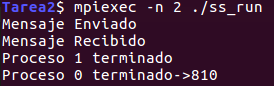
\includegraphics[scale = 0.7]{1.png}
  \label{fig:1}
  \caption{Resultados del Ssend}
\end{figure}


\section{Blocking Ready Send}

El segundo proceso envia la señal de listo para recibir y se bloquea hasta que el primer proceso envie el mensaje.
El código se muestra a continuación y los resultados en la figura \ref{fig:2}

\begin{lstlisting}
#include <stdio.h>
#include <stdlib.h>
#include <time.h>
#include <mpi.h>


int main(){
	srand(time(NULL));
	int id;
	MPI_Init(NULL,NULL);
	MPI_Comm_rank(MPI_COMM_WORLD,&id);
	if(id != 0){
		int random = rand() % 1000;
		int i = 0;
		printf("Mensaje Enviado\n");
		MPI_Rsend(&random,1,MPI_INT,0,0,MPI_COMM_WORLD);
		i += 10;
		i -= 5;
		printf("Proceso 1 terminado\n");
	}
	else{
		int res;
		MPI_Recv(&res,1,MPI_INT,1,0,MPI_COMM_WORLD,MPI_STATUS_IGNORE);
		printf("Mensaje Recibido\n");
		res += 10;
		res -= 5;
		printf("Proceso 0 terminado->%d\n",res);
	}
	MPI_Finalize();
	return 0;
}
\end{lstlisting}

\begin{figure}
  \centering
  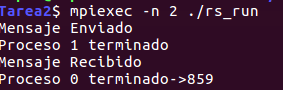
\includegraphics[scale = 0.7]{2.png}
  \label{fig:2}
  \caption{Resultados del Rsend}
\end{figure}

\section{Blocking Buffered Send}

El usuario crea un buffer en donde el mensaje del primer proceso es almacenado; el primer proceso no se bloquea. Cuando el
segundo proceso envia la señal de listo para recibir, el buffer transimite el mensaje. El código se muestra a continuación y
los resultados en la figura \ref{fig:3}

\begin{lstlisting}
#include <stdio.h>
#include <stdlib.h>
#include <time.h>
#include <mpi.h>


int main(){
	srand(time(NULL));
	int id;
	MPI_Init(NULL,NULL);
	MPI_Comm_rank(MPI_COMM_WORLD,&id);
	if(id != 0){
		int random = rand() % 1000;
		int i = 0;
		void * buffer;
		int buffsize = sizeof(int) +  (2 * MPI_BSEND_OVERHEAD);
		buffer = (void *) malloc(buffsize*sizeof(void));
		MPI_Buffer_attach(buffer,buffsize);
		printf("Mensaje Enviado\n");
		MPI_Bsend(&random,1,MPI_INT,0,0,MPI_COMM_WORLD);
		i += 10;
		i -= 5;
		printf("Proceso 1 terminado\n");
	}
	else{
		int res;
		MPI_Recv(&res,1,MPI_INT,1,0,MPI_COMM_WORLD,MPI_STATUS_IGNORE);
		printf("Mensaje Recibido\n");
		res += 10;
		res -= 5;
		printf("Proceso 0 terminado->%d\n",res);
	}
	MPI_Finalize();
	return 0;
}
\end{lstlisting}

\begin{figure}
  \centering
  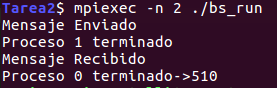
\includegraphics[scale = 0.7]{3.png}
  \label{fig:3}
  \caption{Resultados del Bsend}
\end{figure}

\section{Blocking Standard Send}

El MPI tiene un buffer interno con un tamaño fijo. Si el tamaño del mensaje es menor que el tamaño del buffer, el Standard Send
se comporta como un Buffered Send; pero si el tamaños del mensaje supera el tamaño del buffer, el Standard Send se comporta
como un Synchronous Send. El código se muestra a continuación y los resultados en la figura  \ref{fig:4}

\begin{lstlisting}
#include <stdio.h>
#include <stdlib.h>
#include <time.h>
#include <mpi.h>


int main(){
	srand(time(NULL));
	int id;
	MPI_Init(NULL,NULL);
	MPI_Comm_rank(MPI_COMM_WORLD,&id);
	if(id != 0){
		int random = rand() % 1000;
		int i = 0;
		printf("Mensaje Enviado\n");
		MPI_Send(&random,1,MPI_INT,0,0,MPI_COMM_WORLD);
		i += 10;
		i -= 5;
		printf("Proceso 1 terminado\n");
	}
	else{
		int res;
		MPI_Recv(&res,1,MPI_INT,1,0,MPI_COMM_WORLD,MPI_STATUS_IGNORE);
		printf("Mensaje Recibido\n");
		res += 10;
		res -= 5;
		printf("Proceso 0 terminado->%d\n",res);
	}
	MPI_Finalize();
	return 0;
}
\end{lstlisting}

\begin{figure}
  \centering
  
\includegraphics[scale = 0.7]{4.png}
  \label{fig:4}
  \caption{Resultados del Send}
\end{figure}

\end{document}
